%  A simple AAU report template.
%  2015-05-08 v. 1.2.0
%  Copyright 2010-2015 by Jesper Kjær Nielsen <jkn@es.aau.dk>
%
%  This is free software: you can redistribute it and/or modify
%  it under the terms of the GNU General Public License as published by
%  the Free Software Foundation, either version 3 of the License, or
%  (at your option) any later version.
%
%  This is distributed in the hope that it will be useful,
%  but WITHOUT ANY WARRANTY; without even the implied warranty of
%  MERCHANTABILITY or FITNESS FOR A PARTICULAR PURPOSE.  See the
%  GNU General Public License for more details.
%
%  You can find the GNU General Public License at <http://www.gnu.org/licenses/>.


%  2015-05-08 v. 1.2.0
%  Copyright 2010-2015 by Jesper Kjær Nielsen <jkn@es.aau.dk>
%
%  This is free software: you can redistribute it and/or modify
%  it under the terms of the GNU General Public License as published by
%  the Free Software Foundation, either version 3 of the License, or
%  (at your option) any later version.
%
%  This is distributed in the hope that it will be useful,
%  but WITHOUT ANY WARRANTY; without even the implied warranty of
%  MERCHANTABILITY or FITNESS FOR A PARTICULAR PURPOSE.  See the
%  GNU General Public License for more details.
%
%  You can find the GNU General Public License at <http://www.gnu.org/licenses/>.
%
\documentclass[11pt,oneside,a4paper,openany]{report}
%%%%%%%%%%%%%%%%%%%%%%%%%%%%%%%%%%%%%%%%%%%%%%%%
% Language, Encoding and Fonts
% http://en.wikibooks.org/wiki/LaTeX/Internationalization
%%%%%%%%%%%%%%%%%%%%%%%%%%%%%%%%%%%%%%%%%%%%%%%%
% Select encoding of your inputs. Depends on
% your operating system and its default input
% encoding. Typically, you should use
%   Linux  : utf8 (most modern Linux distributions)
%            latin1 
%   Windows: ansinew
%            latin1 (works in most cases)
%   Mac    : applemac
% Notice that you can manually change the input
% encoding of your files by selecting "save as"
% an select the desired input encoding. 
\usepackage[utf8]{inputenc}
% Make latex understand and use the typographic
% rules of the language used in the document.
\usepackage[danish,english]{babel}
% Use the palatino font
\usepackage[sc]{mathpazo}
\linespread{1.05}         % Palatino needs more leading (space between lines)
% Choose the font encoding
\usepackage[T1]{fontenc}
%%%%%%%%%%%%%%%%%%%%%%%%%%%%%%%%%%%%%%%%%%%%%%%%
% Graphics and Tables
% http://en.wikibooks.org/wiki/LaTeX/Importing_Graphics
% http://en.wikibooks.org/wiki/LaTeX/Tables
% http://en.wikibooks.org/wiki/LaTeX/Colors
%%%%%%%%%%%%%%%%%%%%%%%%%%%%%%%%%%%%%%%%%%%%%%%%
% load a colour package
\usepackage[table]{xcolor}
\definecolor{aaublue}{RGB}{33,26,82}% dark blue
% The standard graphics inclusion package
\usepackage{graphicx}
% Set up how figure and table captions are displayed
\usepackage{caption}
\captionsetup{%
  font=footnotesize,% set font size to footnotesize
  labelfont=bf % bold label (e.g., Figure 3.2) font
}
% Make the standard latex tables look so much better
\usepackage{array,booktabs}
% Enable the use of frames around, e.g., theorems
% The framed package is used in the example environment
\usepackage{framed}

%%%%%%%%%%%%%%%%%%%%%%%%%%%%%%%%%%%%%%%%%%%%%%%%
% Mathematics
% http://en.wikibooks.org/wiki/LaTeX/Mathematics
%%%%%%%%%%%%%%%%%%%%%%%%%%%%%%%%%%%%%%%%%%%%%%%%
% Defines new environments such as equation,
% align and split 
\usepackage{amsmath}
% Adds new math symbols
\usepackage{amssymb}
% Use theorems in your document
% The ntheorem package is also used for the example environment
% When using thmmarks, amsmath must be an option as well. Otherwise \eqref doesn't work anymore.
\usepackage[framed,amsmath,thmmarks]{ntheorem}

%%%%%%%%%%%%%%%%%%%%%%%%%%%%%%%%%%%%%%%%%%%%%%%%
% Page Layout
% http://en.wikibooks.org/wiki/LaTeX/Page_Layout
%%%%%%%%%%%%%%%%%%%%%%%%%%%%%%%%%%%%%%%%%%%%%%%%
% Change margins, papersize, etc of the document
\usepackage[
  inner=28mm,% left margin on an odd page
  outer=41mm,% right margin on an odd page
  ]{geometry}
% Modify how \chapter, \section, etc. look
% The titlesec package is very configureable
\usepackage{titlesec}
\titleformat{\chapter}[display]{\normalfont\huge\bfseries}{\chaptertitlename\ \thechapter}{20pt}{\Huge}
\titleformat*{\section}{\normalfont\Large\bfseries}
\titleformat*{\subsection}{\normalfont\large\bfseries}
\titleformat*{\subsubsection}{\normalfont\normalsize\bfseries}
%\titleformat*{\paragraph}{\normalfont\normalsize\bfseries}
%\titleformat*{\subparagraph}{\normalfont\normalsize\bfseries}

% Clear empty pages between chapters
\let\origdoublepage\cleardoublepage
\newcommand{\clearemptydoublepage}{%
  \clearpage
  {\pagestyle{empty}\origdoublepage}%
}
\let\cleardoublepage\clearemptydoublepage

% Change the headers and footers
\usepackage{fancyhdr}
\pagestyle{fancy}
\fancyhf{} %delete everything
\renewcommand{\headrulewidth}{0pt} %remove the horizontal line in the header
\fancyhead[RE]{\small\nouppercase\leftmark} %even page - chapter title
\fancyhead[LO]{\small\nouppercase\rightmark} %uneven page - section title
\fancyhead[LE,RO]{\thepage} %page number on all pages
% Do not stretch the content of a page. Instead,
% insert white space at the bottom of the page
\raggedbottom
% Enable arithmetics with length. Useful when
% typesetting the layout.
\usepackage{calc}

%%%%%%%%%%%%%%%%%%%%%%%%%%%%%%%%%%%%%%%%%%%%%%%%
% Bibliography
% http://en.wikibooks.org/wiki/LaTeX/Bibliography_Management
%%%%%%%%%%%%%%%%%%%%%%%%%%%%%%%%%%%%%%%%%%%%%%%%
%\usepackage[backend=bibtex,
%  bibencoding=utf8
%  ]{biblatex}
%\addbibresource{references}

%%%%%%%%%%%%%%%%%%%%%%%%%%%%%%%%%%%%%%%%%%%%%%%%
% Misc
%%%%%%%%%%%%%%%%%%%%%%%%%%%%%%%%%%%%%%%%%%%%%%%%
% Add bibliography and index to the table of
% contents
%\usepackage[nottoc]{tocbibind}
% Add the command \pageref{LastPage} which refers to the
% page number of the last page
\usepackage{lastpage}
% Add todo notes in the margin of the document
\usepackage[
%  disable, %turn off todonotes
  colorinlistoftodos, %enable a coloured square in the list of todos
  textwidth=\marginparwidth, %set the width of the todonotes
  textsize=scriptsize, %size of the text in the todonotes
  ]{todonotes}
\usepackage[tocindentauto]{tocstyle}
\usepackage[super]{nth}

%%%%%%%%%%%%%%%%%%%%%%%%%%%%%%%%%%%%%%%%%%%%%%%%
% Hyperlinks
% http://en.wikibooks.org/wiki/LaTeX/Hyperlinks
%%%%%%%%%%%%%%%%%%%%%%%%%%%%%%%%%%%%%%%%%%%%%%%%
% Enable hyperlinks and insert info into the pdf
% file. Hypperref should be loaded as one of the 
% last packages
\usepackage{hyperref}
\hypersetup{%
	pdfpagelabels=true,%
	plainpages=false,%
	pdfauthor={Author(s)},%
	pdftitle={Title},%
	pdfsubject={Subject},%
	bookmarksnumbered=true,%
	colorlinks=false,%
	citecolor=black,%
	filecolor=black,%
	linkcolor=black,% you should probably change this to black before printing
	urlcolor=black,%
	pdfstartview=FitH%
}
\usepackage{tabularx}
\usepackage{makecell}

% Draft watermark
%\usepackage{draftwatermark}
%\SetWatermarkText{DRAFT}
% package inclusion and set up of the document
% see, e.g., http://en.wikibooks.org/wiki/LaTeX/Formatting#Hyphenation
% for more information on word hyphenation
\hyphenation{ex-am-ple hy-phen-a-tion short}
\hyphenation{long la-tex}% 
%  A simple AAU report template.
%  2015-05-08 v. 1.2.0
%  Copyright 2010-2015 by Jesper Kjær Nielsen <jkn@es.aau.dk>
%
%  This is free software: you can redistribute it and/or modify
%  it under the terms of the GNU General Public License as published by
%  the Free Software Foundation, either version 3 of the License, or
%  (at your option) any later version.
%
%  This is distributed in the hope that it will be useful,
%  but WITHOUT ANY WARRANTY; without even the implied warranty of
%  MERCHANTABILITY or FITNESS FOR A PARTICULAR PURPOSE.  See the
%  GNU General Public License for more details.
%
%  You can find the GNU General Public License at <http://www.gnu.org/licenses/>.
%
%
%
% see, e.g., http://en.wikibooks.org/wiki/LaTeX/Customizing_LaTeX#New_commands
% for more information on how to create macros

%%%%%%%%%%%%%%%%%%%%%%%%%%%%%%%%%%%%%%%%%%%%%%%%
% Macros for the titlepage
%%%%%%%%%%%%%%%%%%%%%%%%%%%%%%%%%%%%%%%%%%%%%%%%
%Creates the aau titlepage
\newcommand{\aautitlepage}[2]{%
  {
    %set up various length
    \ifx\titlepageleftcolumnwidth\undefined
      \newlength{\titlepageleftcolumnwidth}
      \newlength{\titlepagerightcolumnwidth}
    \fi
    \setlength{\titlepageleftcolumnwidth}{0.5\textwidth-\tabcolsep}
    \setlength{\titlepagerightcolumnwidth}{\textwidth-2\tabcolsep-\titlepageleftcolumnwidth}
    %create title page
    \thispagestyle{empty}
    \noindent%
    \begin{tabular}{@{}ll@{}}
      \parbox{\titlepageleftcolumnwidth}{
        
\includegraphics[width=\titlepageleftcolumnwidth]{figs/apl_small_vertical_blue.pdf}
      } &
      \parbox{\titlepagerightcolumnwidth}{\raggedleft\sf\small
        #2
      }\bigskip\\
       #1 &
      \parbox[t]{\titlepagerightcolumnwidth}{%
      }\\
    \end{tabular}
    \clearpage
  }
}

%Create english project info
\newcommand{\englishprojectinfo}[4]{%
  \parbox[t]{\titlepageleftcolumnwidth}{
    \textbf{Title:}\\ #1\bigskip\par
    \textbf{Project Participants:}\\ #2\bigskip\par
    \textbf{Authors:}\\ #3\bigskip\par
    \textbf{Date:}\\ #4
  }
}


%%%%%%%%%%%%%%%%%%%%%%%%%%%%%%%%%%%%%%%%%%%%%%%%
% An example environment
%%%%%%%%%%%%%%%%%%%%%%%%%%%%%%%%%%%%%%%%%%%%%%%%
\theoremheaderfont{\normalfont\bfseries}
\theorembodyfont{\normalfont}
\theoremstyle{break}
\def\theoremframecommand{{\color{gray!50}\vrule width 5pt \hspace{5pt}}}
\newshadedtheorem{exa}{Example}[chapter]
\newenvironment{example}[1]{%
		\begin{exa}[#1]
}{%
		\end{exa}
}
% my new macros

\usepackage{xspace}
\usepackage{times}
\usepackage{epsfig}
\usepackage{graphicx}
\usepackage{amsmath}
\usepackage{amssymb}
\usepackage{booktabs}
\usepackage{paralist}
\usepackage{textcase}
\usepackage{float}
\usepackage{subcaption}
\usepackage{stackengine}

\newcommand{\figref}[1]{Figure~\ref{#1}}
\newcommand{\secref}[1]{Section~\ref{#1}}

\newcommand{\eg}{e.g.,\xspace}
\newcommand{\APL}{JHU/APL\xspace}
\newcommand*\rot{\rotatebox{90}}

\newcommand{\subsubheaderbf}[1]{\mbox{\textbf{#1}\hspace*{2.5mm}}}
\newcommand{\subsubheaderit}[1]{\mbox{\textit{#1}\hspace*{2.5mm}}}
\newcommand{\subsubheadertt}[1]{\mbox{\texttt{#1}\hspace*{2.5mm}}}
\newcommand{\subsubheader}[1]{\mbox{#1\hspace*{2.5mm}}}

\begin{document}
%frontmatter
\pagestyle{empty} %disable headers and footers
\pagenumbering{roman} %use roman page numbering in the frontmatter
\pdfbookmark[0]{Title}{label:titlepage_en}
\aautitlepage{%
  \englishprojectinfo{
    Lifelong Learning Machines \\ Metrics Framework \& \\ Proposed Metrics
  }{%
  	\APL Test \& Evaluation Team
  }{%
    Megan Baker \\
    Gautam Vallabha \\ 
  }{%
    \today % date of completion
  }%
}{%department and address
  \textbf{\APL}\\
  \href{http://www.jhuapl.edu/}{http://www.jhuapl.edu/}
}

\cleardoublepage
\pdfbookmark[0]{Contents}{label:contents}
\pagestyle{fancy} %enable headers and footers again
\tableofcontents
%mainmatter
\pagenumbering{arabic} %use arabic page numbering in the mainmatter
\chapter{Background}\label{ch:background}

In this document we introduce the Metrics component of the Test and Evaluation Framework (TEF) for Agent-based evaluation \textit{only.} For this preliminary information release, we focus on a high level overview of the system, followed by a brief introduction to the types of syllabi and metrics which are expected, and end with how to get started with the code. Stay tuned for more details in each of these areas!

\section{Core Capabilities}
\label{sec:core_capabilities}

We remind readers that the purpose of the metrics discussed in this document are to determine whether a system exhibits the Core Capabilities of Lifelong Learning. These metrics may be slightly different from those which might assess a traditional learner. We invite our audience to review the five Core Capabilities whose definitions are below, and refer readers to the BAA for more details.\\%\footnote{DARPA L2M Broad Agency Announcement (April 12 2017)}
\\
\textbf{1. Continual Learning}\\

Ability to handle, or adapt to, changing input distributions (or noise characteristics) within a single task. For an agent-based system, this means that the state transition matrix and reward function are substantively unchanged, while aspects of the environment may change.\\
\\
\textbf{2. Adapting to New Tasks}\\

Ability to learn new tasks, without losing knowledge of already-learned tasks. If possible, system should exploit similarities between old and new tasks to improve its learning performance on new tasks. For an agent-based system, this means substantial changes to the state transition matrix or reward function.\\
\\
\textbf{3. Selective Plasticity}\\

Ability to process the same input differently depending on task (or goal). Relatedly, the ability to be sensitive to different features of the input depending on task. Note the focus on processing rather than learning per se.\\
\\
\textbf{4. Goal-Driven Perception}\\

Ability to incorporate system and task-level constraints (e.g., overall memory use, relative importance of tasks) into the training process.\\
\\
\textbf{5. Safety}\\

Ability to incorporate explicit (failsafe) safety constraints into system performance; Ability to detect differences between training and test environments (e.g., anomalous inputs, distributional shifts), quantify the resulting uncertainty in system output, alert a human operator (with details of difference if possible), and safely handle the anomalous situation where possible.


\section{This Document's Focus}

For the purpose of this initial development, we chose to focus our attention on the first two Core Capabilities; Continual Learning and Adapting to New Tasks. 

\subsection*{Terminology}



\textit{Key Concepts}
\\
Task: A single abstract capability (or skill) that a performer system must learn\\
Episode: A concrete instance of a task\\
Syllabus: A sequence of episodes\\
Learning Lifetime: One syllabus or multiple syllabi in sequence\\
\\
\textit{Metric Specific Terms for Syllabus Design}\\
Phase: A subcomponent of a syllabus during which either training or evaluation takes place\\
Block: A unique combination of task and parameters. It is a subcomponent of phase that is automatically assigned by the logging code and does not need to be annotated by the syllabus designer.\\

% footnote example : \footnote{\url{http://www.es.ele.tue.nl/cvpm18/}}
% citation example : \cite{verkruysse2008remote} 
%\subsection*{Example subsection}
%Subsection related work.

\chapter{System Architecture}\label{ch:system_architechture}

The Syllabus is run, logs are generated, Metrics code is run.



Metrics code scrapes the logs, extracts the relevant information and produces a set of numbers which are used to evaluated each Core Capability





\begin{figure}[h]
	\centering
	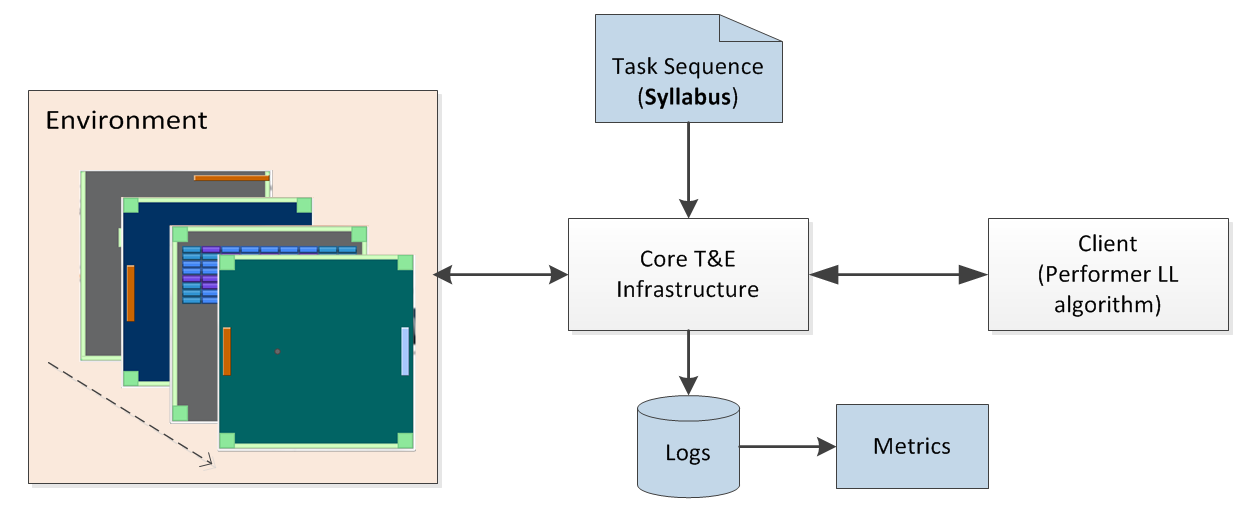
\includegraphics[width=0.85\columnwidth]{sections/figs/metrics_diagram.png}
	\caption{This figure describes the production of Metrics from Log files outputted by the Core Test and Evaluation Framework.}
	\label{fig:system_layout}
\end{figure}



\begin{figure}[h]
	\centering
	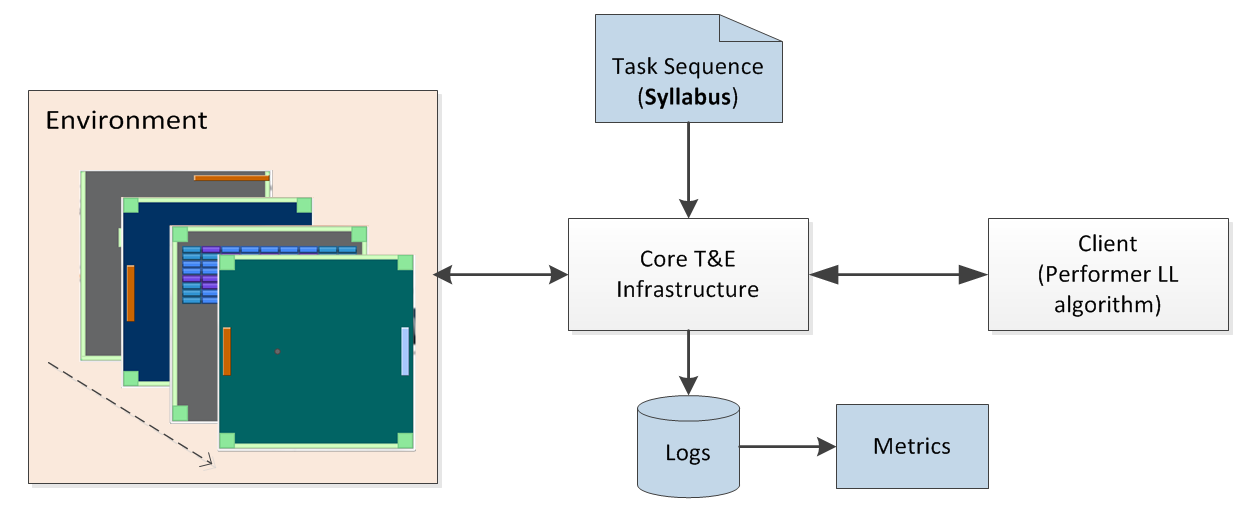
\includegraphics[width=0.85\columnwidth]{sections/figs/metrics_diagram.png}
	\caption{An example log file.}
	\label{fig:system_layout}
\end{figure}

\chapter{Syllabus Types}\label{ch:syllabus_and_metric_types}

With the Core Capabilties in mind, we move on to intentional design of the syllabi. We remind our audience that the calculation of L2M metrics seeks to answer a question that may differ from traditional reinforcement learning evaluation criteria, and thus, we enforce a rigid structure to evaluation tasks.

\section{Term Definitions}

- Phase
    - A phase is
    - Phase number should be incremented, starting with phase 1
    - Phase type can be either "train" or "test"\\
- Block
    - A block is a unique combination of task and parameters. It is a subcomponent of phase that is automatically assigned by the logging code and does not need to be annotated by the syllabus designer.\\
- Task
    - ADD DEFINITION FROM RELEASED DOCUMENTATION HERE\\
- Episode
    - ADD DEFINITION FROM RELEASED DOCUMENTATION HERE\\
    
\section{Syllabus Types by Core Capability} 


\textit{Continual Learning}

    1) This syllabus consists of a single task with parametric variations (P1, P2, P3, ...)\\
        Can involve interpolation of parameters, noisy parameters, etc. but has only one task\\
    2) Each phase consists of a training block and an optional evaluation block\\
        Training block is training on one or more parametric variations \\
        Evaluation block allows Type II metrics to be computed\\
        
    Question: Can the agent adjust to changes in the environment?\\
        Metric: Recovery time (relative to previously trained parameter baseline)\\
            Calculated within and across training blocks \\
            After variation is introduced, does performance fall? Does it recover to the previous level? How quickly does it recover?\\
    
    Question: Can the agent maintain performance on previously learned parameters after being trained with new ones?\\
        Metric: Performance on previously learned parameters\\
            Recommended to be calculated within evaluation block\\

\textit{Adaptation to New Tasks}

    This syllabus consists of multiple, distinct tasks  (T1, T2, T3, ...). Parametric variations within a task are only exercised in Subtype C\\
    Each phase consists of a training block and an evaluation block\\
        Training block is training on one task at a time, and can be over some parametric variation, but only in Subtype C\\
        Evaluation block allows Type B metrics to be computed\\

    Subtype A: No expectation of skill transfer\\
        Parametric variations within a task are not exercised.\\
            Question: Can the agent learn a new task without forgetting the old task?\\
                Metric: Recovery time (relative to previous task baseline)\\
                    Calculated within and across training blocks \\
                    After a new task is introduced, does performance fall? Does it recover to the previous level? How quickly does it recover? \\
                Metric: Performance (reward statistics) on previously learned tasks\\
                    Calculated within evaluation blocks\\
                    Note that this is not to assess forward or reverse transfer; transfer is assessed in ANT Subtype B\\
                    
    Subtype B: Assess basic skill transfer\\
        Parametric variations within a task are not exercised.\\
        Question: Does the agent transfer knowledge from a learned task to a new task?\\
            Metric: Recovery time (relative to previous task baseline)\\
                Calculated within and across training blocks \\
                After a new task is introduced, does performance fall? Does it recover to the previous level? How quickly does it recover? \\
            Metric: Performance (reward statistics) on previously learned tasks\\
                Calculated within evaluation blocks\\
                Note that this is not to assess forward or reverse transfer; transfer is assessed in ANT Subtype B\\
        Metrics are:\\
            Time (number of episodes) to achieve threshold performance on Task 2 after being trained on Task 1\\
            Transfer matrix\\
            
    Subtype C: with Parametric skill transfer\\
        Syllabus has: Parametric variation in Task 1 and then see if that transfers to parametric variation in task 2.\\
        L2Arcade Example: vary paddle width in Pong; does this transfer to varying paddle width in Breakout? \\
            this can be formulated in both a forward and reverse transfer.\\
        Questions\\
            Transfer of general ability: does parametric variation in Pong improve Breakout time-to-learn at all\\
            Transfer of continual learning: Does parametric variation (continual learning) in Pong improve continual learning in Breakout?\\
        Metrics are:\\
            Amount of time required to learn vs from scratch \\
            
\iffalse           
    Compositional skill transfer
        we see this as an instance of 3c 
            Hava mentioned this as a prime goal for L2M program.
            Concern
                How do we identify the "skill relationships" between the tasks? Do we need to do this before designing the syllabus?
            Motivation: system learns Tasks T1, T2, T3 (each having one or more "skills"). Then in T4, system has to use a combination of skills from the prior tasks.
            What this might mean in case of L2Arcade
                T1 = Pong (skills: paddle control, intercept ball, steer ball away from opposing paddle)
                T2 = Breakout (skills: paddle control, intercept ball, steer ball toward blocks)
                T3 = Freeway (skills: control ball, avoid blocks)
                T4 = PongBreakout (skills: paddle control, intercept ball, steer ball toward blocks, and away from opposing paddle)
\fi

\section{Metric Definitions}

1. Saturation Value
    - Purpose: The saturation value is computed to quantify the maximum maintained value by the agent.\\
    - Calculated by: Since multiple rewards may be logged per episode, the mean is taken per episode. Then, the max of the rolling average is taken of the mean reward per episode with a smoothing parameter, s (default, 0.1)\\
    - Compared to: Future or single task expert saturation values of the same task\\
    - Computed for: CL, ANT\_A, ANT\_B\\                   

2. Time to Saturation
    - Purpose: Time to saturation is used to quantify how quickly, in number of episodes, the agent took to achieve the saturation value computed above.\\
    - Calculated by: The first time the saturation value (or above) is seen, that episode number is recorded\\
    - Compared to: Future times to saturation of the same task\\
    - Computed for: CL, ANT\_A, ANT\_B\\

3. Normalized Integral of Reward/Time
    - Purpose: Taking the Integral of Accumulated Reward over Time allows for a more robust comparison of the time to learn a particular task, taking into account both the shape and saturation of the learning for future comparison. Has limitations; must be normalized by length; only training phases can be compared to each other \\
    - Calculated by: Integrating reward over time, then dividing by the number of episodes used to accumulate the reward\\
    - Compared to: Future training instances of this metric\\
    - Computed for: ANT\_B\\

4. Recovery Time
    - Purpose: Recovery time is calculated to determine how quickly (if at all) an agent can "bounce back" after a change is introduced to its environment\\
    - Calculated by: After some training phase achieves a saturation value, determine how many episodes, if any, it takes for the agent to regain the same performance on the same task\\
    - Compared to: An agent's recovery time is comparable across tasks\\
    - Computed for: CL\\

5. Performance Maintenance on Test Sets\\
    - Purpose: Performance maintenance on test sets is calculated to determine whether an agent catastrophically forgets a previously learned task\\
    - Calculated by: Comparing all computed metrics on the train set (saturation values, time to saturation, etc) on the test set and computing the difference in performance\\
    - Compared to: N/A\\
    - Computed for: CL, ANT\_A, ANT\_B\\

6. Performance relative to STE (training) - Saturation Value, Time, Integral\\
    - Purpose: STE Relative performance assesses whether a lifelong learner outperforms a traditional learner.\\
    - Calculated by: Normalizing metrics computed on the lifelong learner by the same metrics computed on the traditional learner\\
    - Compared to: N/A\\
    - Computed for: CL, ANT\_A, ANT\_B\\

7. Forward Transfer (cross tasks)
    - Purpose: Forward transfer assesses whether an agent transfers knowledge from a learned task to a new task\\ 
    - Calculated by:\\ 
    - Compared to: STE performance\\
    - Computed for: CL, ANT\_A, ANT\_B\\
    
8. Forward Transfer (cross tasks)
    - Purpose: Forward transfer assesses whether an agent transfers knowledge from a learned task to a new task\\
    - Calculated by:\\
    - Compared to: STE performance\\
    - Computed for: CL, ANT\_A, ANT\_B\\

9. Time to Learn (cross tasks)
    - Purpose: Time to learn (cross tasks) assesses whether parametric variation in learning task 1 improve time to learn in task 2\\
    - Calculated by: \\
    - Compared to:\\
    - Computed for: ANT-C\\
    
10. Time to Continually Learn (cross tasks)
    - Purpose: Time to continually learn (cross tasks) assesses whether learning task 1 \\
    - Calculated by: \\
    - Compared to:\\
    - Computed for: ANT-C\\


\section{Example Syllabi}

Put up some JSON files here

\chapter{Metrics Code}\label{ch:metrics_code}

\section{Code Release}

L2Metrics code is being released to GitHub! Download it here: \textit{Put a link here}

\subsection{Overview} 

In l2metrics/core.py we introduce an abstract Metric class which describes the general format for any Metric you may use or write, whether for Agent or Classification Learners. The most relevant piece of the Metric class is the calculate method, which has the following required arguments: the log data, a phase\_info dataframe, and a metrics\_dict dataframe. The metrics\_dict starts blank and is filled by each metric in its turn, whereas the log data and the phase info are extracted in the MetricsReport constructor from the logs via two helper functions: \\[0.1in]

l2metrics/util.py - (read\_log\_data): scrapes the logs and returns a pandas dataframe of the logs and task parameters\\
l2metrics/\_localutil.py - (parse\_blocks): builds a pandas dataframe of the phase information contained in the log data\\[0.1in]

These dataframes are passed along by the MetricsReport to the appropriate metric and thus the Metrics and MetricsReport classes should be utilized in conjuction with each other. Though there are a list of default metrics which the MetricsReport uses for the Core Capabilties being exercised at this time, you may choose to add your own metric to this list by using the add method on MetricsReport. Please see the calc\_metrics.py file for more details on how to get started with writing your own custom metric. An extremely simple whole-syllabus-mean is currently implemented as an example to help get you started.


\subsection*{Syllabus and Log Files - Assumptions and Requirements}

\textit{Please note:} Log files should be generated automatically and should require no action on the performer's part. However, Single Task Expert JSON files and/or custom syllabi creation rules must be followed or the L2Metrics code may not work.\\[0.1in]


1. Log files \textbf{must} include logged reward, and the column in the data file \textbf{must} be named reward. Without this column, the metrics code will fail. This is assumed to be logged per episode. \\[0.1in]

2. Single Task Expert Saturation values for each task \textbf{must} be included in a JSON file found in \$L2DATA/taskinfo/info.json and without this file, the metric "Comparison to STE" cannot be calculated. Further, the task names contained in the JSON file must match the names in the log files exactly. The format for this file will be: \\[0.1in]

    \{\\
    "task\_name\_1" : 0.8746,\\
    "task\_name\_2" : 0.9315,\\
    ...,\\
    "task\_name\_n" : 0.8089\\
    \}\\[0.1in]

3. Syllabi used to generate the log files \textbf{must} include annotations with phase information and shall conform to the below convention. Please see Figure~\ref{fig:syllabus} for an example\\[0.1in]

\textit{Phase annotation format}:\\[0.1in]
    \{"\$phase":  "1.train"\}, \{"\$phase":  "1.test"\}, \{"\$phase":  "2.train"\}, \{"\$phase":  "2.test"\}, etc\\[0.1in]

\textit{Structure - Continual Learning}:\\[0.1in]

Consists \textbf{only} of a single task with parametric variations exercised throughout the syllabus. Testing phase is optional, but recommended. The purpose of this type of syllabus is to assess whether the agent can adjust to changes in the environment and maintain performance on the previous parameters when new ones are introduced


\subsection*{Getting Started}

Get started by first generating some log files. You may do this by the following:

1. Download and install the minigridkit repo, located here: \textit{PUT A LINK HERE}

2. Configure your environment variable \$L2DATA to wherever you want your logs to end up.

3. Run minigrid\_learnkit/minigrid\_train\_ppo.py

4. Your logs should appear in \$L2DATA\textbackslash logs\textbackslash  "YOUR\_LOG\_DIRECTORY"\\[0.1in]


Then, you should be able to:\\[0.1in]


5. Pass "YOUR\_LOG\_DIRECTORY" as the log\_dir parameter in the calc\_metrics.py file, and you should get an output printed to console that looks something like this: 


\begin{figure}[h]
	\centering
	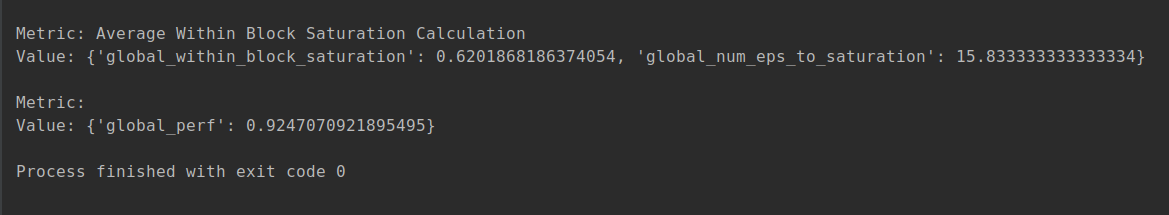
\includegraphics[width=0.85\columnwidth]{sections/figs/calc_metrics_output.png}
	\caption{Sample output for the example calc\_metrics.py .}
	\label{fig:calcmetricsoutput}
\end{figure}

\end{document}
